\section{CurryTest: A Tool for Testing Curry Programs}
\label{sec-currytest}

CurryTest\index{CurryTest}\index{testing programs}\index{program!testing}
is a simple tool in the \CYS distribution to write
and run repeatable tests. CurryTest simplifies the task
of writing test cases for a module and executing them.
The tool is easy to use. Assume one has implemented a module \code{MyMod}
and wants to write some test cases to test its functionality,
making regression tests in future versions, etc.
For this purpose, there is a system library \code{Assertion}
(Section~\ref{Library:Assertion}) which
contains the necessary definitions for writing tests.
In particular, it exports an abstract polymorphic type \ccode{Assertion a}
together with the following operations:
\begin{curry}
assertTrue      :: String -> Bool -> Assertion ()
assertEqual     :: String -> a -> a -> Assertion a
assertValues    :: String -> a -> [a] -> Assertion a
assertSolutions :: String -> (a->Success) -> [a] -> Assertion a
assertIO        :: String -> IO a -> a -> Assertion a
assertEqualIO   :: String -> IO a -> IO a -> Assertion a
\end{curry}
The expression \ccode{assertTrue $s$ $b$}
is an assertion (named $s$) that the expression $b$ has the value \code{True}.
Similarly, the expression \ccode{assertEqual $s$ $e_1$ $e_2$}
asserts that the expressions $e_1$ and $e_2$
must be equal (i.e., \code{$e_1$==$e_2$} must hold),
the expression \ccode{assertValues $s$ $e$ $vs$} asserts
that $vs$ is the multiset of all values of $e$,
and the expression \ccode{assertSolutions $s$ $c$ $vs$} asserts
that the constraint abstraction $c$ has the multiset of solutions $vs$.
Furthermore, the expression \ccode{assertIO $s$ $a$ $v$}
asserts that the I/O action $a$ yields the value $v$ whenever it is
executed, and
the expression \ccode{assertEqualIO $s$ $a_1$ $a_2$}
asserts that the I/O actions $a_1$ and $a_2$ yield equal values.
The name $s$ provided as a first argument in each assertion
is used in the protocol produced by the test tool.

One can define a test program by importing the module
to be tested together with the module \code{Assertion} and defining
top-level functions of type \code{Assertion} in this module
(which must also be exported).
As an example, consider the following program
that can be used to test some list processing functions:
\begin{curry}
import List
import Assertion

test1 = assertEqual     "++"     ([1,2]++[3,4]) [1,2,3,4]

test2 = assertTrue      "all"    (all (<5) [1,2,3,4])

test3 = assertSolutions "prefix" (\x -> x++_ =:= [1,2])
                                 [[],[1],[1,2]]
\end{curry}
For instance, \code{test1} asserts that the result of evaluating the
expression \code{([1,2]++[3,4])} is equal to \code{[1,2,3,4]}.

We can execute a test suite by the command\pindex{currytest}
\begin{curry}
currytest TestList
\end{curry}
(\code{currytest} is a program stored in \code{\cyshome/bin}
where \cyshome is the installation directory of \CYS;
see Section~\ref{sec-general}).
In our example, \ccode{TestList.curry} is the program containing the
definition of all assertions. This has the effect
that all exported top-level functions
of type \code{Assertion} are tested (i.e., the corresponding
assertions are checked) and the results
(\ccode{OK} or failure) are reported together with the name of each assertion.
%If failures occur, the complete test results are also
%written into a file named \ccode{TestList.testlog}.''
For our example above, we obtain the following successful protocol:
\begin{curry}
============================================================
Testing module "TestList"...
OK: ++
OK: all
OK: prefix
All tests successfully passed.
============================================================
\end{curry}
There is also a graphical interface that summarizes the results
more nicely.
In order to start this interface, one has to add the parameter
\ccode{--window} (or \ccode{-w}), e.g., executing a test suite by
\begin{curry}
currytest --window TestList
\end{curry}
or
\begin{curry}
currytest -w TestList
\end{curry}
A snapshot of the interface is shown in Figure~\ref{fig-currytest}.

\begin{figure}%[t]
\begin{center}
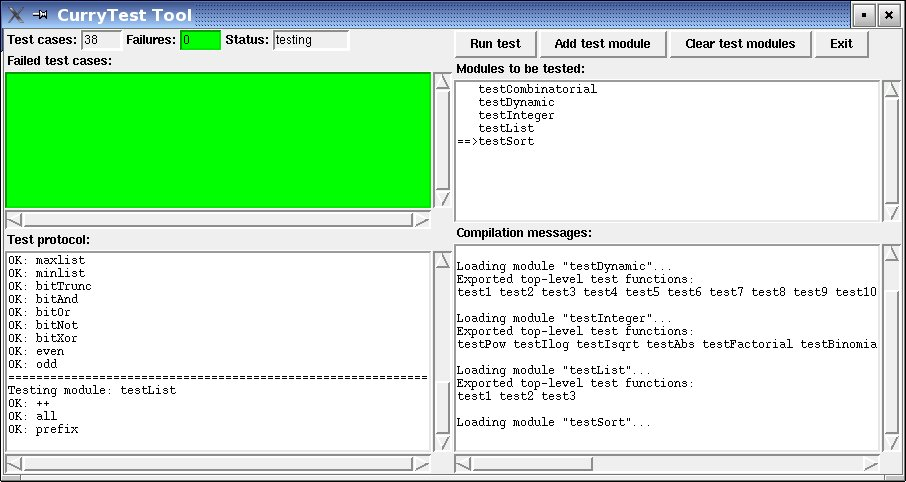
\includegraphics[scale=0.7]{currytest.jpg}
\end{center}
\caption{Snapshot of CurryTest's graphical interface\label{fig-currytest}}
\end{figure}
